\documentclass[a4paper,twoside,twocolumn,10pt]{article}
\usepackage{abstract} % Style for abstracts in Dept. CSIS, OPU
%\usepackage{abstract4past} % Style for abstracts for the past curriculum

%%%%%%%%%% Designate packages you need %%%%%%%%%%
\usepackage[dvipdfmx]{graphicx} % Enhanced support for graphics
\usepackage{url} % Verbatim with URL-sensitive line breaks

%%%%%%%%%% Parameters that should be customized %%%%%%%%%%
% Language (1 = Japanese, 2 = English)
\setlang{1}
% Bachelor or Master (1 = Bachelor, 2 = Master)
\setborm{1}
% Fiscal year
\setfy{2021}
% Group number
\setgnum{1}
% Presentation order
\setorder{1}
% Increase page number (optional)
%% \pplus{1}

% Title
\title{TDGA を導入した DARTS による深層学習の構造探索}
% Author
\author{杉山 竜弥}
%%%%%%%%%% Parameters that should be customized (end) %%%%%%%%%%

\begin{document}
\maketitle % Insert title
\small

\section{はじめに}
機械学習の分野では, 深層学習モデルの改良によって大きく精度が向上してきた.
しかしモデルの設計とその性能の関係はブラックボックスであり
手作業でによるチューニングには膨大な労力を要する.

ネットワークの探索を自動化する手法として提案された
Neural Architecture Search(NAS)はネットワークを機械学習によって探索する.
しかし何千ものGPUを必要とするため, NASに代わり
小規模な資源で計算できるDifferentiable Architecture Search(DARTS)
が大きな注目を集めている.
DARTSはネットワークの構造と演算子の候補を探索するが,
一方でDARTSにはネットワーク構造にいくつかの拘束条件がある.

本研究では演算子の種類ではなくネットワークの構造にのみ着目し,
DARTSの構造制限をなくしネットワークの柔軟な探索を目的とする.
その初期段階として, VGG19のショートカット位置についてDARTSで探索を行う方法を提案する.


\section{要素技術}

\subsection{Differentiable Architecture Search}
Differentiable Architecture Search(DARTS)\cite{DBLP:journals/corr/abs-1806-09055}は,
離散的なアーキテクチャ探索空間に強化学習を適用した NAS with RL とは異なり,
微分可能な方法で定式化し,
偏微分による勾配降下法を使用してアーキテクチャを効率的に探索する手法である.


\subsection{Thermodynamical Genetic Algorithm}
Thermodynamical Genetic Algorithm (TDGA) は熱力学における自由エネルギー最小化をモデルにした,
GAで個体群の多様性を維持する手法である.
選択に温度とエントロピーの概念を導入し, 初期収束問題を解決した.

\section{提案手法}
\subsection{実験1:DARTS}
予備実験としてDARTSを用いてネットワークを探索する手法について様々なパラメータで実験した.

\subsection{実験2:DARTS+TDGA}

実験1では $\alpha$ の学習度によって重み $w$ の学習しやすさに偏りがあったため,
収束するグラフ構造にばらつきが見られた.

そこで個体表現を $\alpha$ とした遺伝的アルゴリズムによって,
アーキテクチャの多様性を維持しつつ, 安定的な
ネットワーク構造の学習を図った.
しかし単純に個体数を増やすと, 計算コストが定数倍されるので,
重み $w$ は全体で共有する One-Shot モデルを利用することで,
高速化した.

\begin{enumerate}
  \item DARTSで事前学習したモデルの重みを引き継いだ初期個体を生成
  \item エリート個体選択
  \item 個体 $\alpha_i$ を $\displaystyle \nabla_\alpha \mathcal{L}_{\mathrm{valid}}(w^*, \alpha_i)$ で更新
  \item 適応度 $\displaystyle \mathcal{L}_{\mathrm{test}}(w, \alpha^\mathrm{smp})$ で個体 $\alpha$ を評価
  \item 交叉で子個体群生成
  \item 親個体群と子個体群の突然変異
  \item エリート個体と親個体, 子個体に熱力学的選択をして次世代とする
  \item 収束するまで 2. に戻る
\end{enumerate}


\section{数値実験}
\subsection{実験1}
Sigmoid関数と閾値によるサンプリング手法が有効であるとわかった.

\subsection{実験2}
実験1から引き継いだモデルの重みを初期値としてTDGAを行ったところ,
探索中は重みを固定することでTDGAが機能し, ベースラインを超えるアーキテクチャが探索できることがわかった.
図 \ref{fig:eval_tdga} では, 50 世代から 150 世代までのネットワークの評価結果を示しており,
TDGAと組み合わせたDARTSが有効に機能していると言える.

\begin{figure}[t]
  % \begin{center}
  %   % 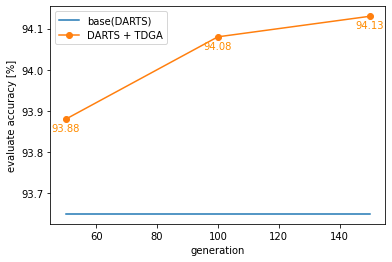
\includegraphics[clip, width=70mm]{eval_tdga.png}
  %   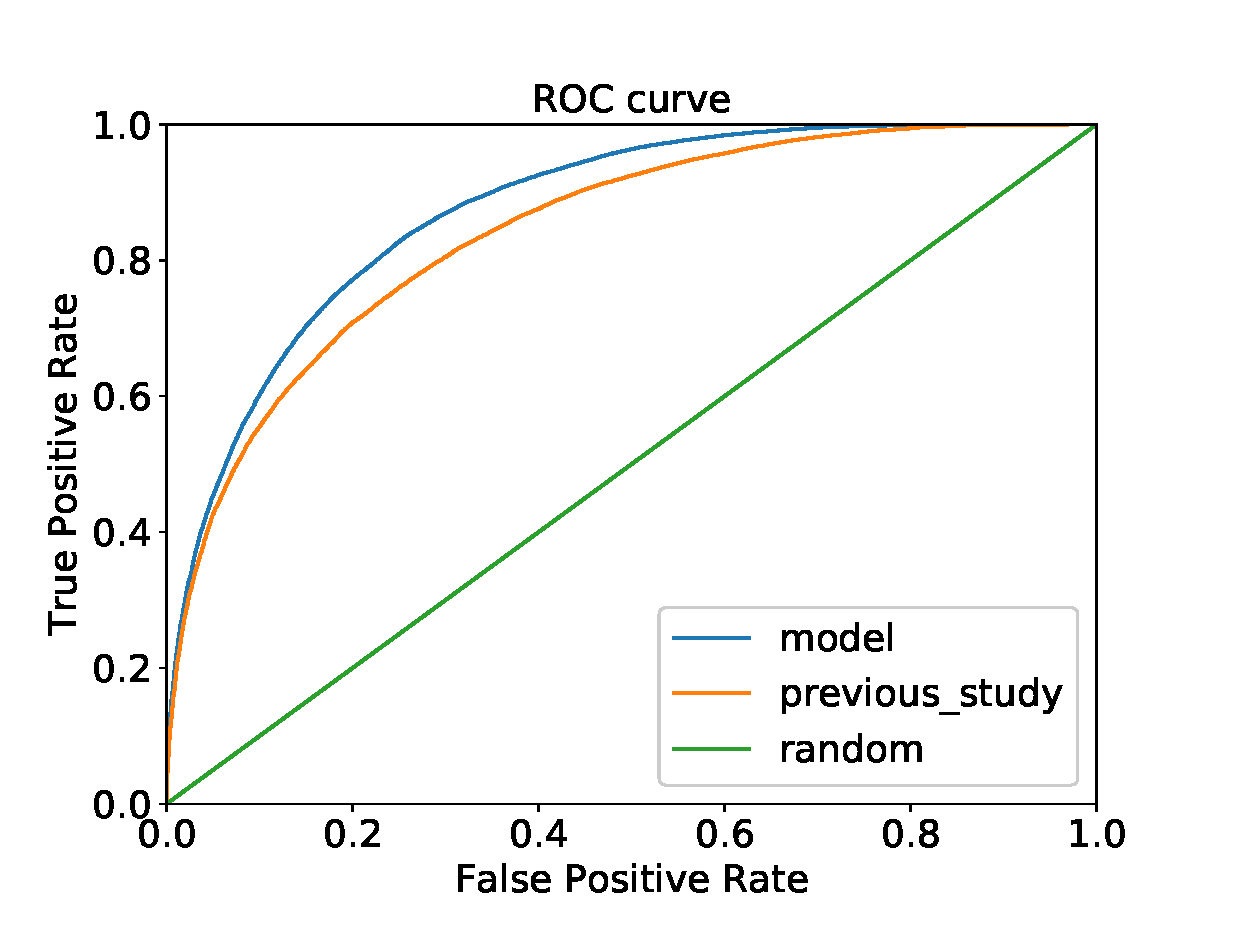
\includegraphics[clip, width=70mm]{ROC_gather.eps}
  % \end{center}
  \centering
  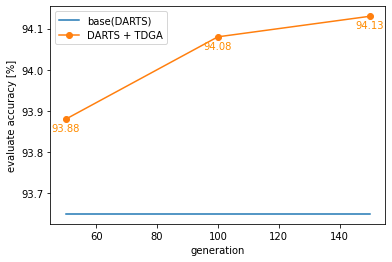
\includegraphics[width=80mm]{eval_tdga.png}
  \caption{TDGA eval}
  \label{fig:eval_tdga}
\end{figure}

% \begin{figure}[tb]
%   \centering
%   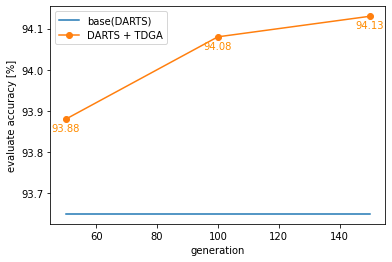
\includegraphics[clip, width=7cm]{eval_tdga.png}
%   \caption{TDGA eval}
%   \label{fig:eval_tdga}
% \end{figure}
%
% \begin{table}[tb]
%   \caption{ROC 曲線の曲線下面積}
%   \label{auc_tenpai}
%   \centering
%   \begin{tabular}{|c||c|} \hline
%   モデル & 曲線下面積 \\ \hline \hline
%   model & 0.8761\\ \hline
%   previous\_study & 0.8430\\ \hline
%   random & 0.5000\\ \hline
%   \end{tabular}
% \end{table}

\section{まとめと今後の課題}
本研究では,
% LSTM によるニューラルネットワークモデルを用いて,従来よりも高精度な他プレイヤのテンパイ予測モデルを構築した.今後の課題としては,今回構築したモデルの予測結果を踏まえた上で最適な捨て牌を決定するモデルの構築が挙げられる.
%
DARTSの欠点であるアーキテクチャ構造の制限を緩和するようなネットワーク探索ができた.

% しかしながらまだネットワークの構成手法は改善の余地がある.
% 選択しないという候補を導入して, 他のショートカットと妥当な比較ができると考えられる.

TDGAを導入することで, ベースラインを超えることができた.

% 今後の課題として, 他のデータセットや実問題に対して提案手法によるアーキテクチャの汎用性を確認したい.
% またパラメータ数が少ないモデルが得られるような適応度の設定についても検討する予定である.

%%%%%%%%%%%%%%%%%%%%%%%%%%%%%%

\bibliographystyle{jabbrvunsrt}
\bibliography{index_ja}
\end{document}
